% Imports
\documentclass[9pt, dvipsnames]{beamer}
\usepackage{times}
\usepackage{amsmath}
\usepackage{amsthm}
\usepackage{verbatim}
\usepackage{anyfontsize}
\usepackage{subcaption}
\usepackage{graphicx}
\usepackage[export]{adjustbox}
\usepackage[multidot]{grffile}
\usepackage{tabularx}
\usepackage{tikz}
\usetikzlibrary{positioning}
\usepackage{wasysym}
\usepackage{amsmath,amssymb,amsfonts}


% Beamer Themes
\definecolor{st}{RGB}{190, 15, 57}
\usetheme{Ilmenau}
\useinnertheme{circles}
\usecolortheme[named=st]{structure}
\usefonttheme{professionalfonts}
\setbeamertemplate{caption}[numbered]

% Counter
\newcounter{saveenumi}
\resetcounteronoverlays{saveenumi}

% Bibliography -- all nocited here in case they don't get inline cited
% \addbibresource{bibliography.bib}
\nocite{groher}
\nocite{angenent}
\nocite{valeri}

% style stuff
\definecolor{tab-blue}{RGB}{31, 119, 180}
\definecolor{tab-red}{RGB}{214, 39, 20}
\definecolor{input}{RGB}{120, 0, 0}
\definecolor{output}{RGB}{210, 0, 0}

\tikzstyle{Input} = [
    rectangle,
    rounded corners=5pt,
    draw,
    thick,
    fill=input,
    text=white,
    text centered,
    minimum width=2cm,
    minimum height=1cm,
]

\tikzstyle{Output} = [
    rectangle,
    rounded corners=5pt,
    draw,
    thick,
    fill=output,
    text=white,
    text centered,
    minimum width=2cm,
    minimum height=1cm,
]

% Preamble
\title[ML in Synth. Bio.]{Explorations of Machine Learning Methodologies to Enhance the Design of RNA-based Dopamine Biosensors}
\author[Abernathys' Group]{James Craven and Matthew Lindsey}
\date{Friday, June 28$^{\text{th}}$ 2024}


\begin{document}


\maketitle

\section{Introduction}
\begin{frame}{Benefits of a Dopamine Sensor}
Dopamine is a neurotransmitter and plays a role in a variety of functions
such as memory, learning, and reward systems. Detecting dopamine levels
could help with diagnosing:
    \begin{itemize}
        \item addiction
        \item mental illness
        \item neurodegenerative disorders
    \end{itemize}
\end{frame}

\begin{frame}{Building a Synthetic Ribosensor}
%Dopamine detection via ribosensor relies on two apatamers bound together: one that binds to dopamine and another that fluoresces. 
\textbf{Research Question:} How can we leverage machine learning to inform the
necessary nucleotide sequence for the designed ribosensor in order for the ribosensor
to emit a strong fluorescence in the presence of dopamine?
\begin{center}
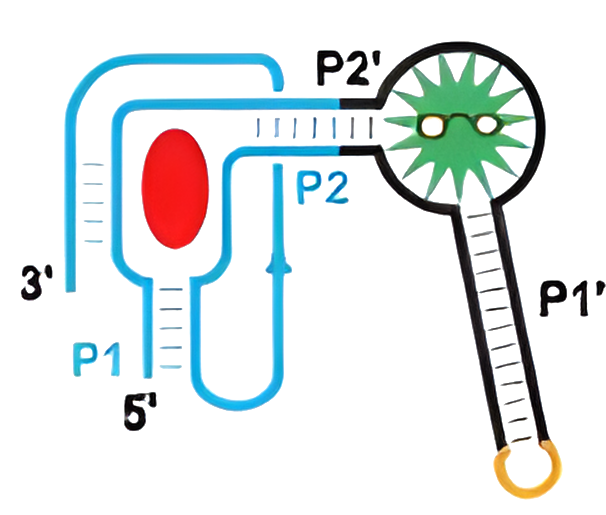
\includegraphics[height=0.3\paperheight]{assets/ribo3.png}
\end{center}
    \small
    \color{ForestGreen}\textellipsis GUCCA
    \color{black} GCUGC 
    \color{cyan} GGAAGAAACUGUGGCACUUCGGUGCCAG
    \color{black} GCAGC
    \color{ForestGreen} UUGU\textellipsis
\end{frame}

\begin{frame}{Data Understanding for ML}
In order to begin building such a model, we first need to understand: 
\begin{itemize}
\item is our data labeled?
\item how much data do we have?
\end{itemize}

\pause
\bigskip

The Fernandez lab supplied us with roughly 15 labeled instances of ribosensor
data, along with labeled data from a literature review of similarly built ribosensors,
for total a dataset of 103 instances.

\pause
\bigskip

While this seems like a healthy amount of experimental data, many machine learning
models need 10-100x that amount to discover relationships between the features and
target of a dataset.
\end{frame}

\begin{frame}{Previous Work}
In an effort to better understand how machine learning is currently used in synthetic
biology, we came across the work of Angenent-Mari et al. \cite{angenent}. Results from
this work include:

\begin{itemize}
\pause
    \item creation of a dataset of over 90,000 toehold switches
    \pause
    \item training of a multilayer perceptron (MLP) to adequately predict
    fluorescence for the toehold switch data
    \pause
    \item the MLP outperforms other regression-based models in predicting fluorescence
    \pause
    \item all models tested performed better when trained on nucleotide sequences
    instead of derived thermodynamic parameters
\end{itemize}

\end{frame}

\begin{frame}{Research Questions}
    Since some of the Fernandez lab ribosensors are riboswitch-like in design,
    our research questions for this work are two-fold:
    \begin{enumerate}
    \pause
    \item Using both the toehold switch dataset and the Fernandez lab data, do
    models perform better when trained on nucleotide sequences than thermodynamic
    parameters? Additionally, does the MLP outperform other regression-based models
    for both datasets?
    \pause
    \item Can we leverage the 90,000+ labeled toehold switch dataset to train a ML
    model and make accurate predictions on the Fernandez ribosensor data?
    \end{enumerate}
\end{frame}

\section{Preparing the Data}

\begin{frame}{Handling Sequences}
    Most machine learning models require the input data to have the same dimensionality.
    An option to handle sequences of variable length is to pad them to the same length.
    \\ \pause
    \vspace{.25in}
        \textellipsis GUAGAGUGUGAGCUCCGUAACUAGUCGCGUC  \\ \pause
        \begin{center}
        $\downarrow$
        \end{center}
        \textellipsis GUAGAGUGUGAGCUCCGUAACUAGUCGCGUC{\color{st} AUAUAUAUAUAUAUAU}
\end{frame}

\begin{frame}{Handling Sequences}
    In addition, sequence data has to be adequately formatted before being used to
    train a machine learning model. Plain-text characters can't be used directly. \\
    \vspace{.25in}
    \begin{center}
        
\begin{tikzpicture}
            \node[Input] (sequences) {GUCCAGCUGC\textellipsis};
            \onslide<2-> {
                \node[Input, right=1cm of sequences, fill=white, text=black] (label) {2311021321};
                \draw[thick, ->] (sequences) -- (label);
            }
            \onslide<3-> {
                \node[Output, right=1cm of label] (onehot) {[0 0 1 0], [0 0 0 1], \textellipsis};
                \draw[thick, ->] (label) -- (onehot);
            }
        \end{tikzpicture}
    \end{center}
\end{frame}

\begin{frame}{Data Preparation for Model Building}
    \begin{itemize}
        \item The two data sets also have two distinct target values, namely
        fold increase and on/off ratio. \pause
        \item To properly compare the results of the data sets, these two values
        were normalized using range-based normalization.
        \pause
        \item With the data preprocessed, we trained and cross-validated seven
        regression-based models on the nucleotide sequence and thermodynamic parameters
        separately for both datasets.
    \end{itemize}
\end{frame}

\section{Modeling}
\begin{frame}{Constructing Regression Models}
    \begin{center}
        \begin{figure}[hp!]
        \centering
        \subfloat[Linear Regression]{%       
            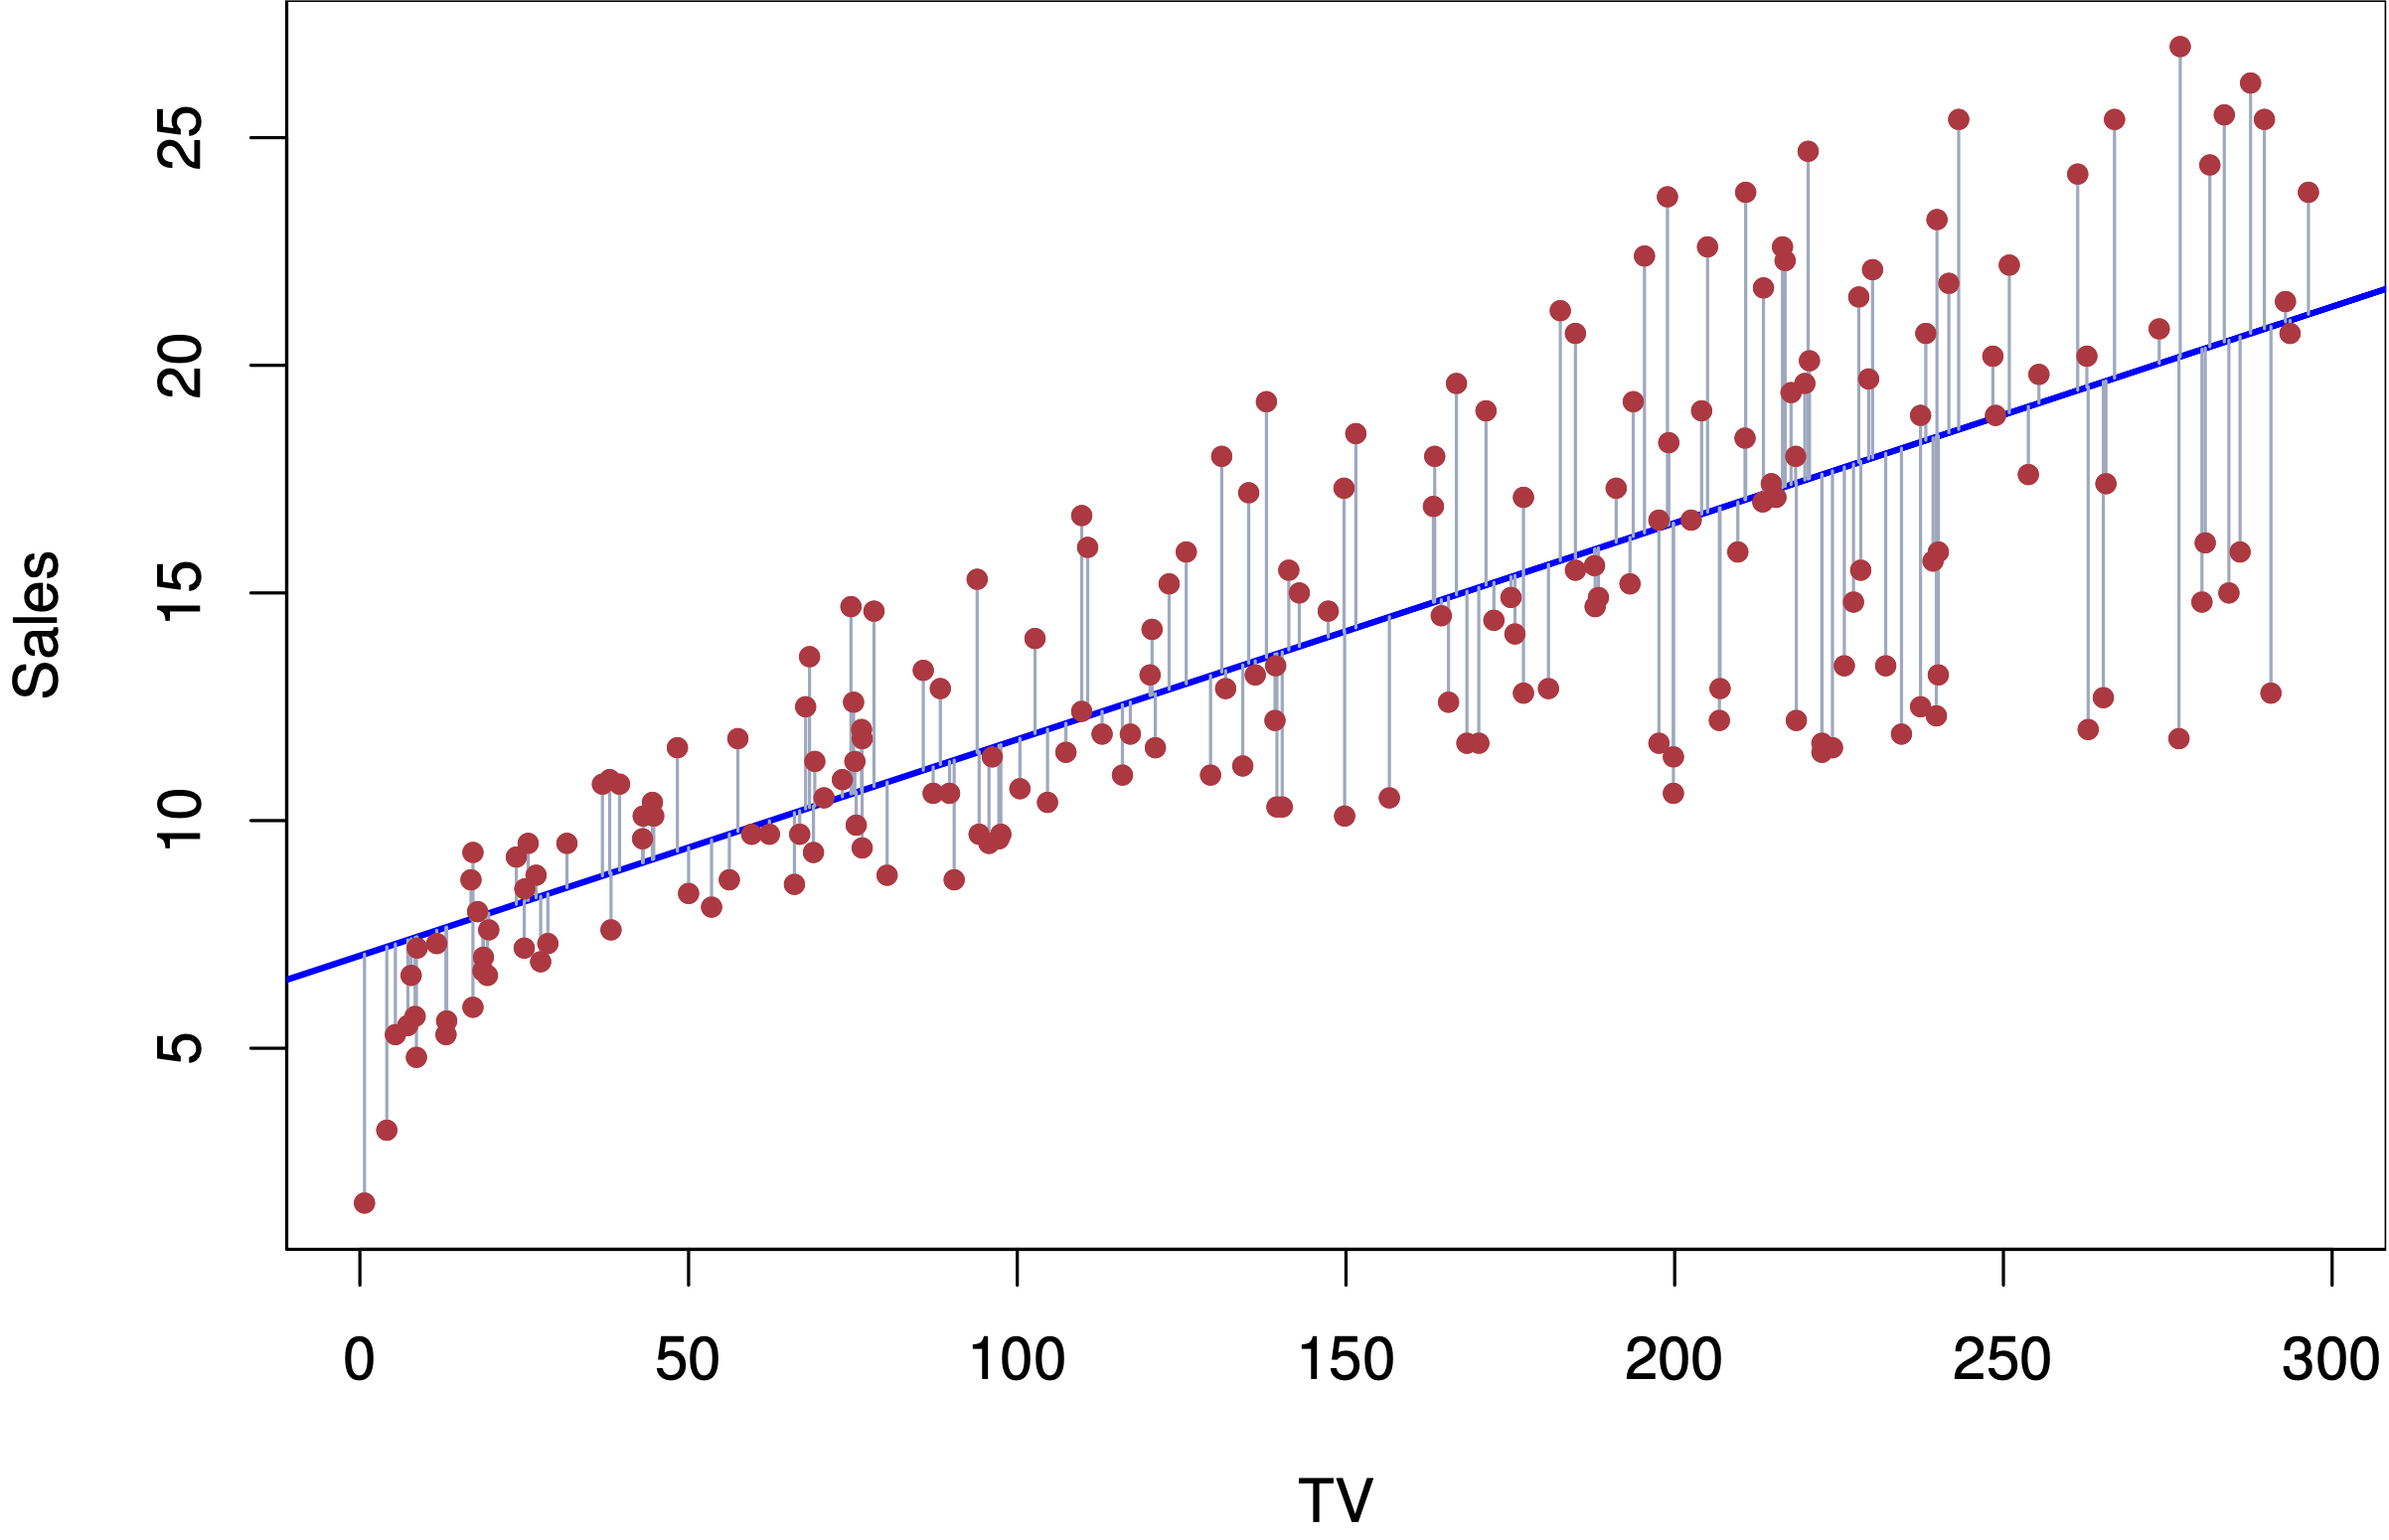
\includegraphics[width=0.45\textwidth, height=2.5cm]{assets/regression.png}
        }\hfill  \pause      
        \subfloat[Decision Tree]{%
            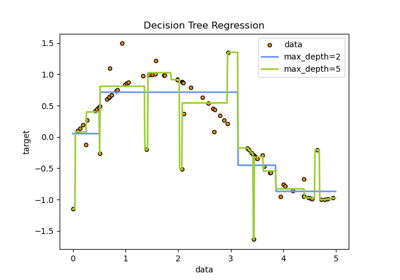
\includegraphics[width=0.45\textwidth, height=2.5cm]{assets/decision-tree.png}
        }\\         \pause
        \subfloat[Support Vector Machine]{%       
            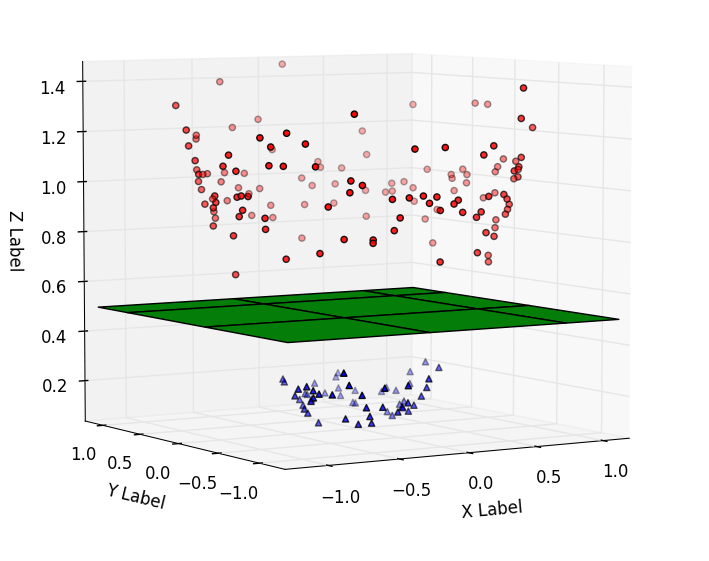
\includegraphics[width=0.45\textwidth, height=2.5cm]{assets/support-vector-machine.png}
        }\hfill       \pause 
        \subfloat[Neural Network]{%
            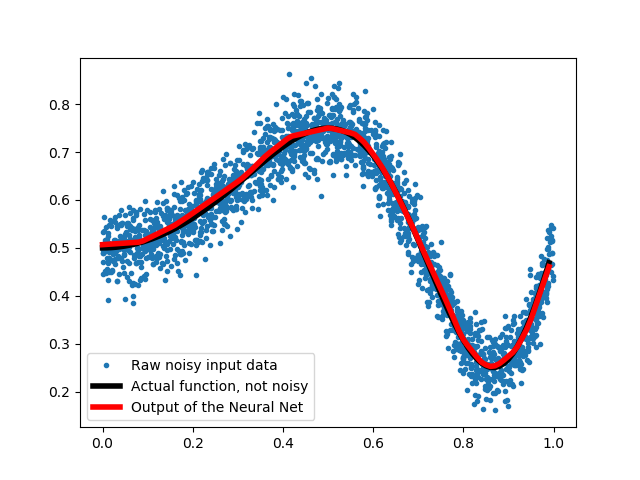
\includegraphics[width=0.45\textwidth, height=2.5cm]{assets/neural-netwrok-regression.png}               
        }
        \end{figure} 
    \end{center}
\end{frame}

\section{Evaluation}

\begin{frame}{A Metric for Comparing Regression Models}

    We utilize scikit-learn's implementation of the coefficient of determination:

    \[R^2(y,\hat{y}) = 1 - \frac{\sum_{i=1}^n (y_i - \hat{y_i})^2}{\sum_{i=1}^n (y_i - \bar{y})^2}\]
    \pause
    \vspace{.1in}
    \begin{center}
        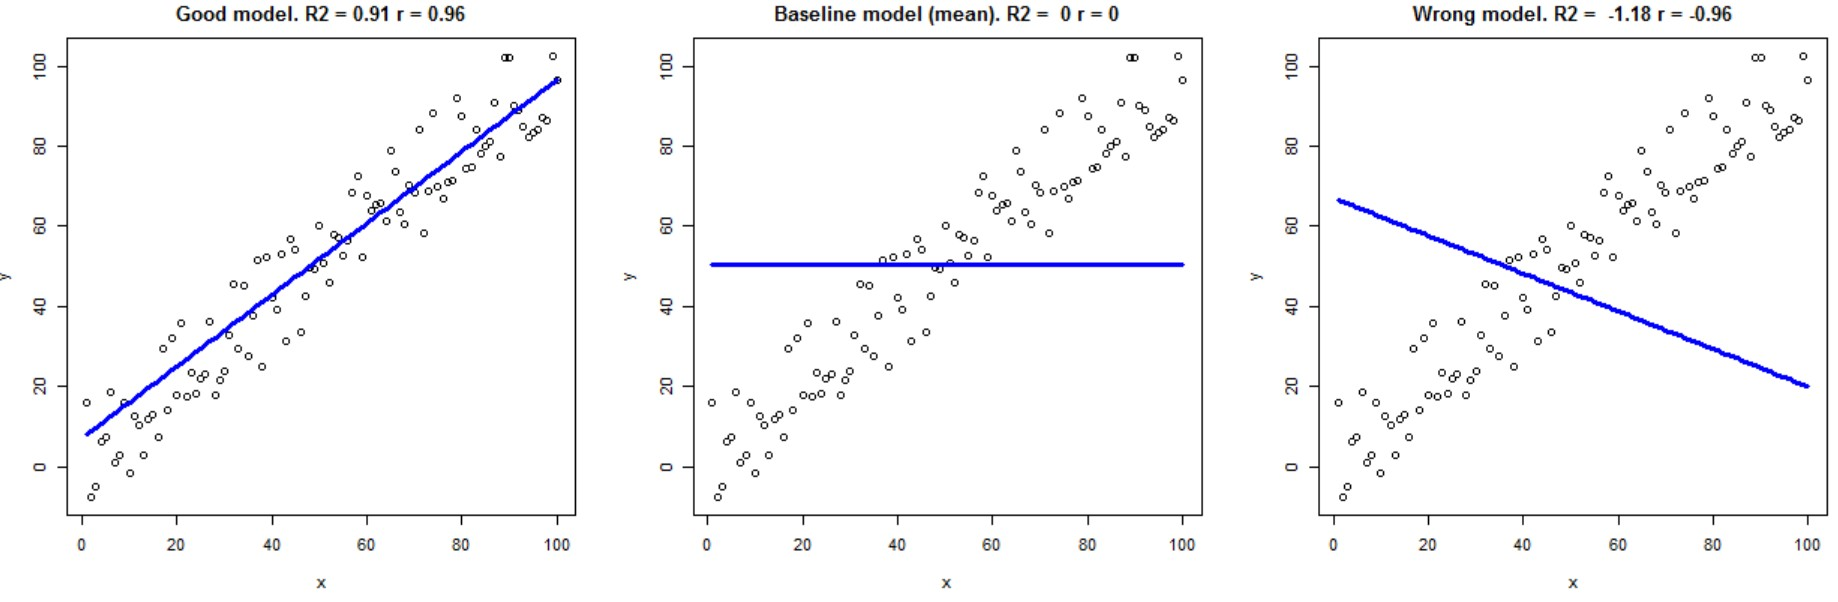
\includegraphics[height=0.3\paperheight]{assets/R2_comparison.jpg}
    \end{center}
\end{frame}

\begin{frame}{Research Question 1}
    \Large
    \begin{itemize}
        \item Using both the toehold switch dataset and the
        Fernandez lab data, do models perform
        better when trained on nucleotide sequences than thermodynamic parameters? 
        \bigskip
        \item Additionally, does the MLP outperform other
        regression-based models for both datasets?
    \end{itemize}
\end{frame}

\begin{frame}{Results for Toehold Switches}
    \begin{center}
        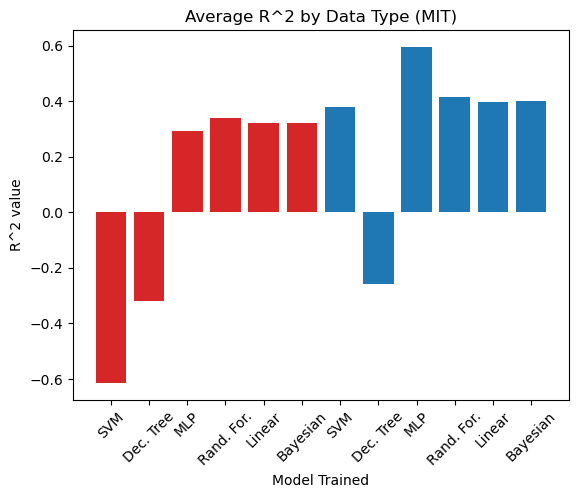
\includegraphics[height=0.7\paperheight]{assets/Average-R^2-by-Data-Type-MIT.png}
    \end{center}
\end{frame}

\begin{frame}{Results for Ribosensor Data}
    \begin{center}
        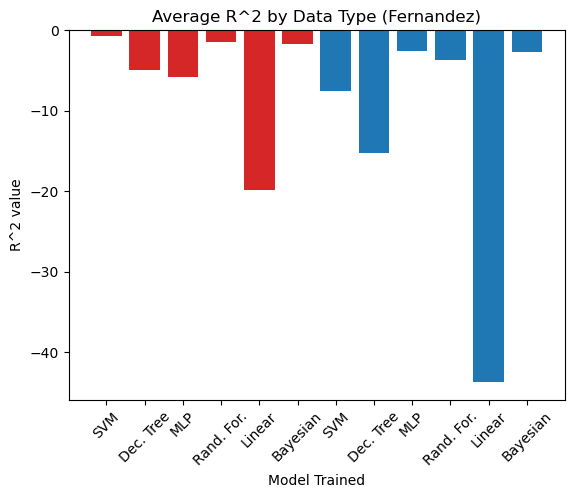
\includegraphics[height=0.7\paperheight]{assets/Average-R^2-by-Data-Type-Fernandez.png}
    \end{center}
\end{frame}

\begin{frame}{Research Question 2}
    \Large
    Can we leverage the 90,000+ labeled toehold switch dataset to train a
    ML model and make accurate predictions on the Fernandez ribosensor data?
    \bigskip
    \pause

    \textbf{Results:} We trained a MLP on the full 90,000+ toehold switch
    dataset and tested on the ribosensor data. In doing so, we obtained an
    $R^2$ score of -0.458.

\end{frame}

\section{Conclusion}
\begin{frame}{Key Accomplishments and Summary of Results}
    \large
    Key Accomplishments:
    \begin{itemize}
        \item Developed framework for one-hot encoding nucleotide
        sequences to train ML models\pause
        \item Created data preprocessing pipeline to pad sequences
        and normalize output values \pause
        \item Constructed neural net model architecture for training
        on both sequence and parameter data
    \end{itemize}
    Summary of Results:
    \begin{itemize}
        \item Sequence data appears to be better for model training due
        to potential information loss in calculating thermodynamic parameters\pause
        \item Neural Networks are effective models for this type
        of problem \pause
        \item There is either not enough similarity between the datasets or
        there is not enough data, in general, to do cross-training between the two
    \end{itemize}
\end{frame}

\begin{frame}{Future Directions of the Project}
\large
    \begin{itemize}
        \item Pre-training the neural net on Harvard data and then unfreezing layers
        and retraining on a portion of Fernandez data\pause
        \item Semi-supervised learning by generating millions of sensor sequences and
        using Large Language Models (LLM) to learn general RNA patterns that can be
        applied to the smaller labeled dataset\pause
        \item Revisiting the literature to see if other data sources are closer
        in design to our dopamine sensors
    \end{itemize}
\end{frame}

\begin{frame}{References}
    \bibliography{bibliography}
    \bibliographystyle{plain}
\end{frame}

\begin{frame}{Acknowledgements}
    \begin{center}
        {\Large \textbf{\color{st} Thanks! Any questions?}} \\
        \bigskip
        
\includegraphics[height=0.2\paperheight]{assets/repo-qr.png} \\
        {\color{st} GitHub} \\
        \bigskip
        { \scriptsize
        This work was supported primarily by the National Science Foundation
        EPSCoR Program under NSF Award \#OIA-2242812. Any Opinions, findings
        and conclusions or recommendations expressed in this material are
        those of the author(s) and do not necessarily reflect those of the
        National Science Foundation.
        }
    \end{center}
\end{frame}


\end{document}